\chapter{Graphs of Sine and Cosine Functions}

Determine the amplitude, period, phase shift, and vertical shift for each. Exact answers only.

\begin{enumerate}
	\item $f(x) = -2\sin\left(3x-\frac{\pi}{4}\right) + 1$
	\item $g(x) = \frac{1}{3}\cos\left(\frac{1}{2}x + 2\right)$
	\item $f(x)=2\sin\left(x-\frac{\pi}{3}\right)+7$
	\item $f(x)=-4\cos\left(\frac{2}{3}x-\frac{2\pi}{3}\right)$
\end{enumerate}
\setcounter{Review}{\value{enumi}}

Write the equation of each of the following in the form $y = a\sin(bx)$.
\begin{multicols}{2}
\begin{enumerate}	\setcounter{enumi}{\value{Review}}
	\item \mbox{} \newline\\ 
	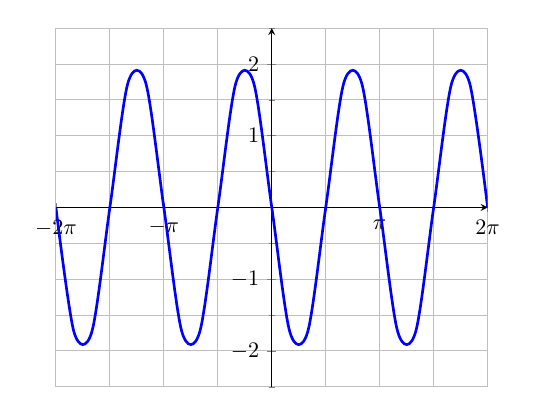
\begin{tikzpicture}[scale=0.8]
    \begin{axis}[
    axis lines = middle, xmin = -2*pi, xmax = 2*pi, ymin=-2.5, ymax=2.5, xtick={-2*pi, -pi, 0, pi, 2*pi}, xticklabels={$-2\pi$, $-\pi$, 0, $\pi$, $2\pi$}, grid=both, minor tick num = 1]
    \addplot[blue, very thick, domain=-2*pi:2*pi, smooth] {-2*sin(2*deg(x))};
    \end{axis}
    \end{tikzpicture}
    
    \item \mbox{} \newline\\
    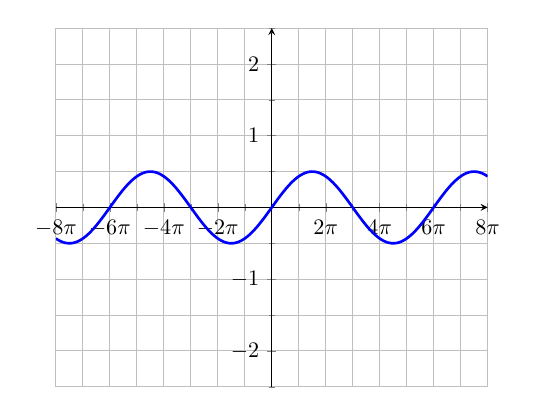
\begin{tikzpicture}[scale=0.8]
    \begin{axis}[
    axis lines = middle, xmin = -8*pi, xmax = 8*pi, ymin=-2.5, ymax=2.5, xtick={-8*pi,-6*pi,-4*pi,-2*pi, 0, 2*pi, 4*pi, 6*pi, 8*pi}, xticklabels={$-8\pi$, $-6\pi$, $-4\pi$, $-2\pi$, 0, $2\pi$, $4\pi$, $6\pi$, $8\pi$}, grid=both, minor tick num = 1]
    \addplot[blue, very thick, domain=-8*pi:8*pi, samples=200] {(1/2)*sin((1/3)*deg(x))};
    \end{axis}
    \end{tikzpicture}
\end{enumerate}
\end{multicols}

\newpage

\textsc{Answers}

\begin{enumerate}
	\item Amp = 2, Per = $\frac{2\pi}{3}$, P.S. = $\frac{\pi}{12} \rightarrow$, V.S. = $1 \uparrow$
    \item Amp = $\frac{1}{3}$, Per = $4\pi$, P.S. = $4 \leftarrow$, V.S. = None
    \item Amp = 2, Period = $2\pi$, P.S. = $\frac{\pi}{3}$ right, V.S. = 7 up
    \item Amp = 4, Period = $3\pi$, P.S. = $\pi$ right, V.S. = 0 (or none)
    
    \item $y = -2\sin(2x)$
	\item $y = \frac{1}{2}\sin\left(\frac{1}{3}x\right)$
\end{enumerate}